\documentclass{beamer}
\mode<presentation>
\usetheme{Frankfurt}

\usepackage{array}
\usepackage{multirow}

\title{Solar Water Heating System with Phase Change Material}
\subtitle{(SWHS)}
\author{Brooks MacLachlan}
\date{\today}

\begin{document}
	
\begin{frame}
	\titlepage
\end{frame}
	
\begin{frame}
	\frametitle{Background info}
	\begin{columns}
	\column{0.5\textwidth}
	\begin{itemize}
	\item Solar energy is a renewable, environmentally friendly alternative to fossil fuels
	\item Regular solar water heating tanks must be large to facilitate the storage of sufficient thermal energy
	\item Phase Change Material (PCM) can store thermal energy in the form of latent heat
	%This means that PCM absorbs/releases large amounts of thermal energy during phase change (i.e. melting/freezing)
	\begin{itemize}
	\item Allows for smaller solar water heating tanks
	\end{itemize}
	\end{itemize}
	\column{0.5\textwidth}
	\begin{figure}[center]
	\includegraphics[scale=0.6]{Tank.png}
	\caption{Simplified diagram of a solar water heating tank}
	%This picture makes the tank look rectangular, but really the software requires for the tank to be cylindrical.
	\end{figure}
	\end{columns}
\end{frame}
	
\begin{frame}
	\frametitle{Purpose of the software}
	The purpose of the software, called Solar Water Heating System (SWHS), is to:
	\begin{itemize}
	\item simulate the charging of a single solar water heating tank incorporating PCM
	%Charging means the period of time where the water heats up, PCM heats and melts and continues heating
	\item predict the temperature and thermal energy profiles of water and PCM
	\item predict the start and end times for the melting process of the PCM
	\end{itemize}
\end{frame}
		
\begin{frame}
	\frametitle{Inputs}
	SWHS accepts a text file containing numerical values for the following parameters:
	\begin{itemize}
	\item Properties of coil:
	\begin{itemize}
	\item Surface area, temperature
	\end{itemize}
	\item Properties of tank:
	\begin{itemize}
	\item Length, diameter
	\end{itemize}
	\item Properties of water:
	\begin{itemize}
	\item Density, specific heat capacity, convective heat transfer coefficient between water and PCM and between water and coil, initial temperature
	\end{itemize}
	\item Properties of PCM:
	\begin{itemize}
	\item Volume, surface area, density, specific heat capacity as solid and as liquid, specific latent heat of fusion, melting temperature, initial temperature (same as water)
	\end{itemize}
	\item Parameters for numerical algorithm:
	\begin{itemize}
	\item time step size, end time, relative tolerance, and absolute tolerance
	\end{itemize}
	\end{itemize}
\end{frame}
	
\begin{frame}
	\frametitle{Outputs}
	Running the SWHS software outputs the following:
	\begin{itemize}
	\item Input parameters, values of temperature and energy throughout simulation time
	\begin{itemize}
	\item Written to text file
	\end{itemize}
	\item Graphs of temperature and energy of water and PCM over time
	\begin{itemize}
	\item Saved as PDF and PNG files
	\end{itemize}
	\item Start and stop times for melting of PCM
	\begin{itemize}
	\item Printed to screen
	\end{itemize}
	\end{itemize}
\end{frame}
	
\begin{frame}
	\frametitle{System Design}
	\framesubtitle{Module Hierarchy}
	The software is divided into modules, which themselves can be sorted into two levels of hierarchy.
		
	\begin{tabular}{ | c | c | p{0.2\textwidth} |}
	\hline
	\textbf{Level 1} & \textbf{Level 2} & \textbf{Implemented by}\\
	\hline
	\multirow{2}{0.25\textwidth}{Hardware Hiding Module} & & \multirow{2}{0.2\textwidth}{OS}\\
	& & \\
	\hline
	\multirow{6}{0.25\textwidth}{Behaviour Hiding Module} & Input Format Module & \multirow{6}{0.2\textwidth}{SWHS}\\
	& Input Parameters Module & \\
	& Output Format Module & \\
	& Temperature ODEs Module & \\
	& Energy Equations Module & \\
	& Control Module & \\
	\hline
	\multirow{3}{0.25\textwidth}{Software Decision Module} & Sequence Data Structure Module & \multirow{3}{0.2\textwidth}{MatLab}\\
	& ODE Solver Module & \\
	& Plotting Module & \\
	\hline
	\end{tabular}
	%See MG or MIS for more info on modules
\end{frame}
	
\begin{frame}
	\frametitle{System Design}
	\framesubtitle{Module Use Hierarchy}
	\begin{figure}
	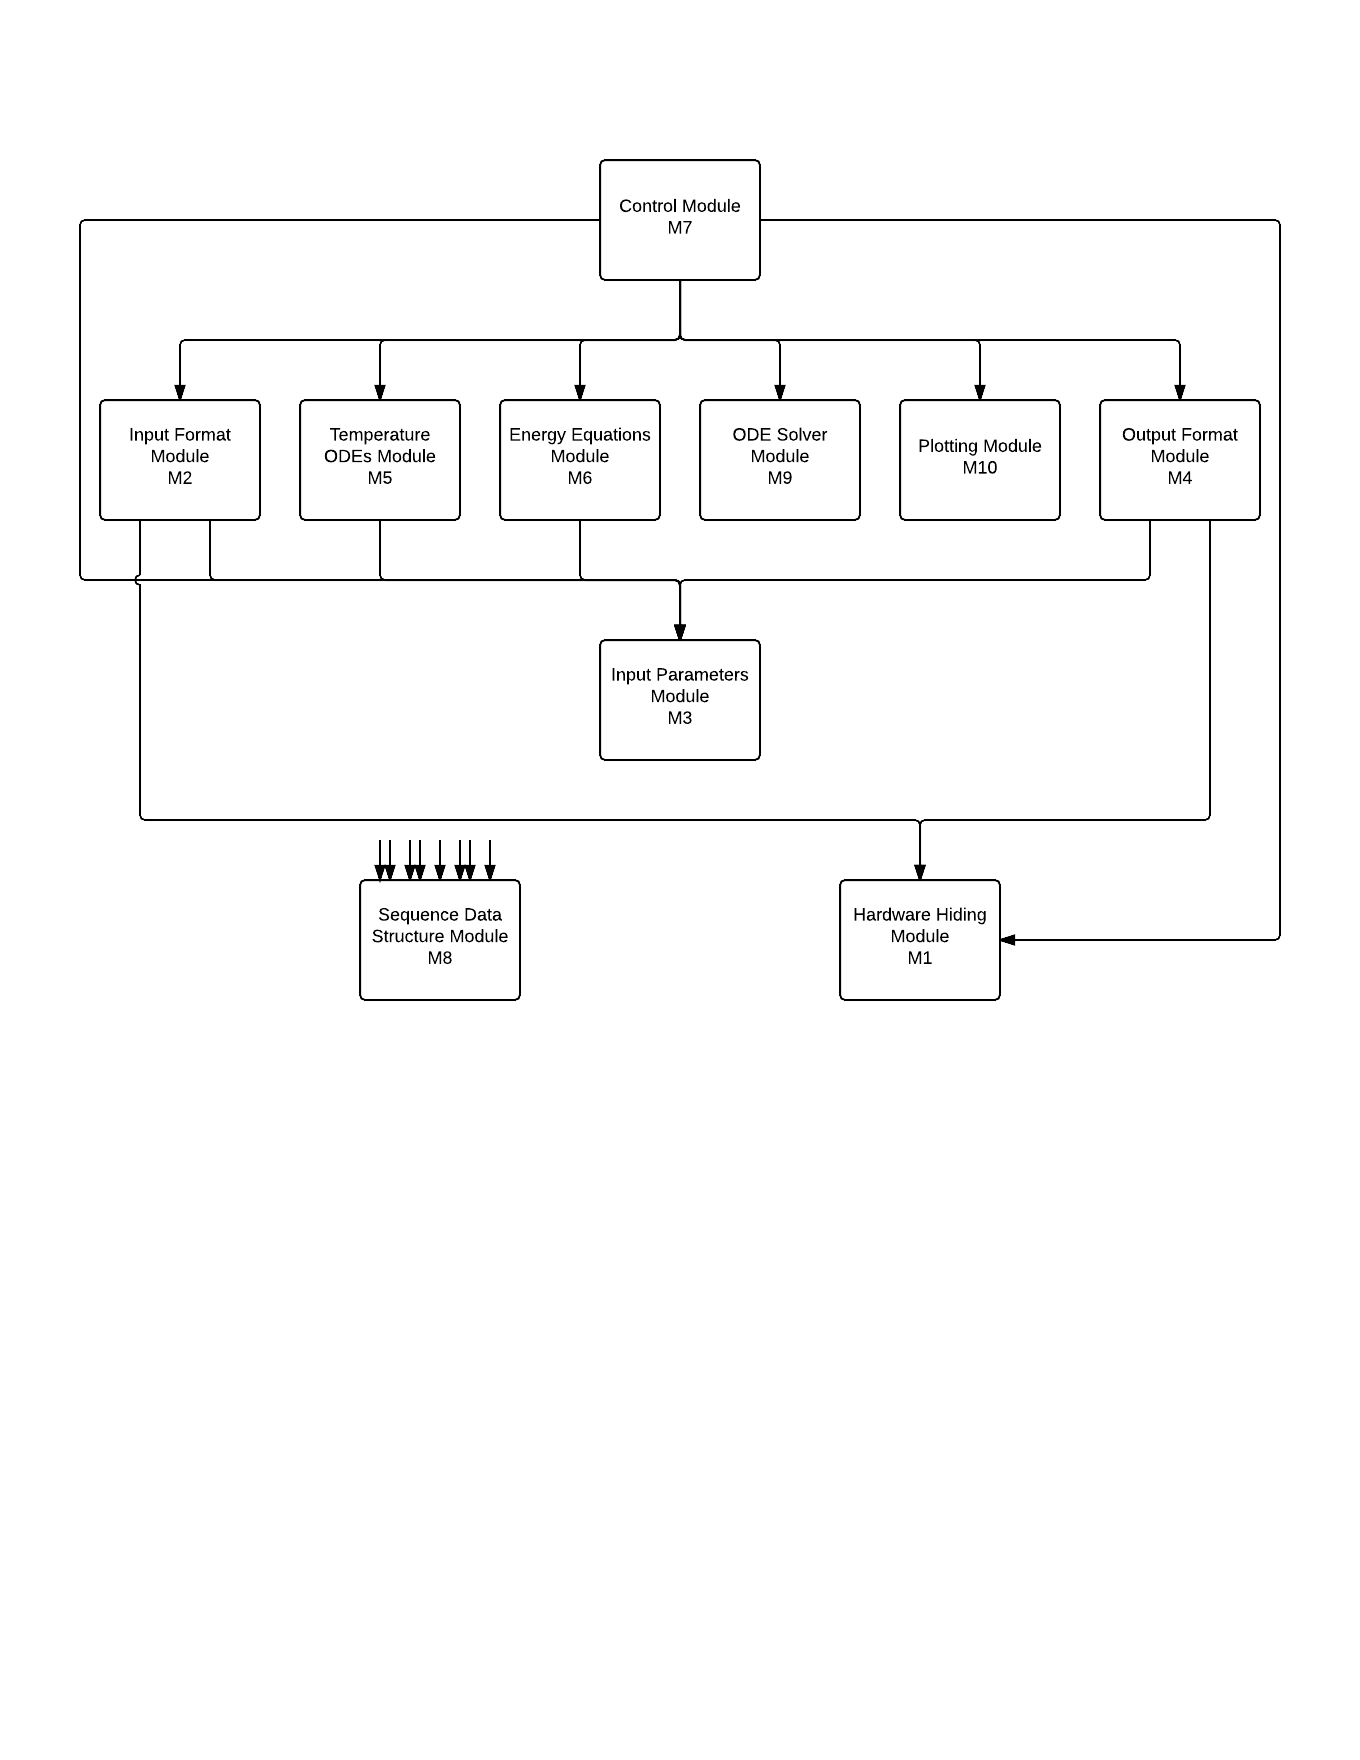
\includegraphics[scale=0.45]{UsesHierarchy.png}
	\end{figure}
\end{frame}
	
\begin{frame}[fragile]
	\frametitle{Running the software}
	The SWHS software was written in MatLab code. The Control Module is implemented by the main.m function. Calling this function in MatLab with the filename for the file containing the input values as the only parameter will run the program.\\
	For example:\\
	~\newline
	\begin{verbatim}
	>> main('test.in')
	PCM has started to melt at time 3322.065744
	PCM has finished melting at time 20571.368997
	>>
	\end{verbatim}
	%test.in is simply a text file of parameters saved as a .in file
\end{frame}
	
\begin{frame}
	\frametitle{Running the Software}
	\framesubtitle{Example output graphs}
	\begin{figure}[center]
	These are an example of the graphs that the function outputs:
	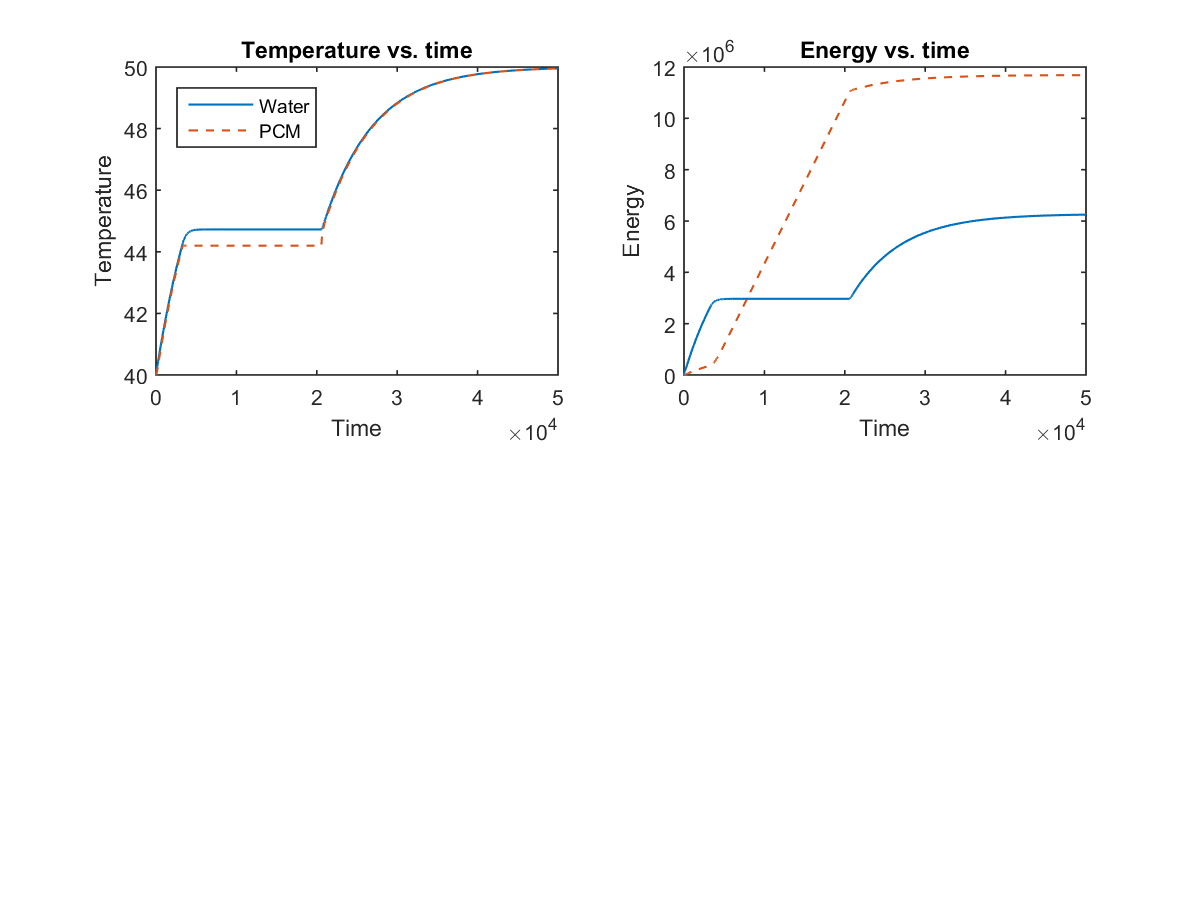
\includegraphics[scale=0.6]{NewTemp.png}
	%Notice the sharp increase in PCM energy during melting (when temperature stays constant)
	\end{figure}
\end{frame}
	
\begin{frame}[fragile]
	\frametitle{Sample Test Cases}
	\framesubtitle{Faulty Input}
	\textbf{Input:}\\
	Standard input with one parameter changed to a value outside of the physical constraints.\\
	%Standard input means all of the parameters set to their "typical" values, as shown in the SRS
	~\newline
	\textbf{Expected Output:}\\
	Error message specific to the faulty parameter.\\
	~\newline
	\textbf{Example:}\\
	~\newline
	\textbf{Input:} Tank length of -2 m, standard input for remaining parameters.\\
	\textbf{Expected Output:} \verb|error: Tank length must be > 0|		
	%Each error is associated with a MsgID, which is what the test case checks to confirm expected output
\end{frame}

\begin{frame}[fragile]
	\frametitle{Sample Test Cases}
	\framesubtitle{Comparisons to Similar Programs}
	\textbf{Example:}\\
	~\newline
	\textbf{Input:} Standard input to both the MatLab implementation of SWHS and the original FORTRAN implementation of the program.\\
	\textbf{Expected Output:} Numerical output values with a relative error of 0.01 between the two versions of the software.\\
	~\newline
	\textbf{Example:}\\
	~\newline
	\textbf{Input:} Standard input to both the current SWHS version and an alternative that uses the \verb|ode23| numerical algorithm for solving ODEs instead of \verb|ode45|.\\
	%ode23 and ode45 are built in MatLab functions for solving ODEs
	\textbf{Expected Output:} Numerical output values with a relative error of 0.01 between the two versions of the software.\\
\end{frame}

\begin{frame}[fragile]
	\frametitle{Sample Test Cases}
	\framesubtitle{Unit Tests}
	\textbf{Example:}\\
	~\newline
	\textbf{Input:} Standard input and a time \verb|t=100| and a temperature vector \verb|T=[44.2, 44.2]| to the event1.m MatLab function.\\
	\textbf{Expected Output:} Row Vector \verb|[0, 1, 0]|\\
	%event functions are part of the temperature ODEs module, and they handle the switch between different modes of heating (pre-melting, during melting, and post-melting). In the row vector result, the second and third elements should always be 1 and 0. When the first element equals zero, it stops the current ODE solver and allows the main.m function to advance to the next set of ODEs.
	~\newline
	\textbf{Example:}\\
	~\newline
	\textbf{Input:} Standard input and a temperature matrix \verb|T=[40:44; 40:44]'| to the energy1.m MatLab function.\\
	%The apostrophe at the end of the temperature matrix tells MatLab to take the transpose of the matrix. This is necessary because the function requires that the temperature matrix has columns representing the different components of the system (i.e. water and PCM)
	\textbf{Expected Output:} Change in energy of water and of PCM, where \verb|Ew1=[0; 627795.094; 1255590.188; 1883385.281; 2511180.375]| and \verb|Ep1=[0; 88616; 177232; 265848; 354464]|\\
\end{frame}

\begin{frame}
	\centering
	\huge Thank you!
\end{frame}

\end{document}